\chapter{Umfeld}
\section{Firmenumfeld}
dSPACE ist der weltweit f\"uhrende Anbieter von L\"osungen f\"ur die Entwicklung und den Test schneller mechatronischer Regelungssysteme. dSPACE-"-Echtzeit-"-Simulationssysteme  erm\"oglichen den Herstellern von Reglern und Steuerger\"aten ihre Entwicklungszeiten und -kosten drastisch zu reduzieren und die Produktqualit\"at zu erh\"ohen. M\"oglich ist dies durch einen aufeinander abgestimmten Mix aus Standardl\"osungen und kundenspezifischem Engineering f\"ur Reglerentwicklung, automatische Seriencode-"-Generierung und automatisierte Systemtests.
Mittlerweile stellen weltweit mehr als 7.000 dSPACE-Systeme ihre Leistungsf\"ahigkeit unter Beweis. \"Uberall dort, wo schnelle Regelungssysteme zum Einsatz kommen, finden sich heute dSPACE Systeme. Neben der Fahrzeugelektronik sind dies vor allem Bereiche wie Antriebstechnik, Luft- und Raumfahrt oder Robotik. Zu den dSPACE Kunden z\"ahlen fast alle Hersteller und Elektronik-Zulieferer der Automobilindustrie, sowie namhafte Unternehmen aus anderen Bereichen, zum Beispiel ABB, Audi, BMW, Bosch, DaimlerChrysler, Delphi, DENSO, Ford, Fujitsu, General Motors, Kodak, Magneti Marelli, Mitsubishi, Philips, PSA, Siemens, Visteon und VW~\cite{dSPACEGmbH.2014b}.

\section{Produktumfeld}
Im Rahmen der Entwicklung von Fahrerassistenzsystemen werden zunehmend kamerabasierte Tests durchgef\"uhrt, bei denen die Echtzeit 3D-Visualisierung von Kamerasystemen aufgenommen und analysiert wird.  Man spricht hierbei von Visualisierung, da das gerenderte Bild auf Daten basiert - zum Beispiel Stra\ss{}eneigenschaften oder G\"ultigkeitsbereichen von Stra\ss{}enschildern. Nach der Aufnahme des Bildes ist eine Echtzeitbildverarbeitung notwendig. Diese wird dabei auf dedizierten \textbf{I}mage \textbf{P}rocessing \textbf{U}nits (\textbf{IPU}) vorgenommen, welche die Erkennung und das Track"-ing von Objekten \"ubernehmen. IPUs senden ihre Trackingdaten an ein oder mehrere Steuerger\"ate (\textbf{E}letronic \textbf{C}ontrol \textbf{U}nits - \textbf{ECU}s), die einen Regelalgorithmus implementieren (z.B. Notbremsung). Gem\"a\ss{} des Algorithmus sendet die ECU Steuersignale an die angeschlossenen Aktuatoren (z.B. Bremsen)~\cite{Meyer.2012}. Diese Verarbeitungskette der Bilddaten ist in Abbildung~\ref{fig:Verarbeitungskette} nochmals skizziert.

\begin{figure}[h!]
\begin{tikzpicture} [
    auto,
    decision/.style = { diamond, draw=dsRed, thick, fill=dsRed!80,
                        text width=1em, text badly centered,
                        inner sep=0.00pt , font=\footnotesize},
    block/.style    = { rectangle, thick, 
    				text width=12em, text centered,text width=2.7cm, draw=dsBlue, fill = dsBlue!20,
                       		 rounded corners, minimum height=7em, font=\footnotesize},
    line/.style     = { draw, thick, ->, shorten >=2pt , font=\footnotesize},
  ]


  \matrix [column sep=0.8cm, row sep=9mm] {
                  
                   	\node [block ](1) {\textbf{Kamera} \singlespace Mono-, Stereo- oder Nachtsichtkamera};    
                   	&            
		\node [block](2) {\textbf{Bildverarbeitung} \\ Objekterkennung und Tracking };                        
				 &
		\node [block](3) {\textbf{Regelalgorithmus} \\ z. B. der Lichtverteilung oder der Notbremsung};       
				 &
		\node [block](4) {\textbf{Aktuator} \\ z. B. der Scheinwerfer oder Bremsen};      



 \\
  };
  % connect all nodes defined above

  % connect all nodes defined above
  \begin{scope} [every path/.style={line, draw=black}]
   \path[latex-latex, ultra thick, dsRed] (1) -- (2);
   \path[latex-latex, ultra thick, dsRed]  (2) -- (3);
   \path[latex-latex, ultra thick, dsRed]  (3) -- (4);
  \end{scope}

\end{tikzpicture}
\caption{Verarbeitungskette kamerabasierter Systeme}
  \label{fig:Verarbeitungskette}
\end{figure}

Um kamerabasierten Systeme zu testen, werden zum einen echtzeitf\"ahige Simulator Hardware (kurz: Simulator) und zum anderen Host-PCs f\"ur die Hardwaresteuerung und die 3D-Visualisierung verwendet. Der Aufbau eines solchen Tests wird in Abbildung~\ref{fig:HiL} schematisch dargestellt. Die zu testende IPU des Fahrerassistenzsystems wird dabei in einem Regelkreis (\textbf{H}ardware \textbf{i}n the \textbf{L}oop-Simulation - \textbf{HIL}) \"uber spezielle I/O Karten am Simulator angeschlossen, wobei die Kamera auf die Ausgabe des 3D-Visualisierung ausgerichtet wird. W\"ahrend der Simulator Fahrverhalten, Umgebung und Fahrman\"over in Echtzeit berechnet und \"uber die 3D-Visualisierung ausgibt, nimmt die Kamera diese auf. Das Bild der Kamera wird von der IPU verarbeitet. Anschließend werden die Trackingdaten der erkannten Objekte an den Simulator oder an eine ECU gesendet und hier weiter verwertet. Falls vorhanden wird die ECU an den Simulator angeschlossen. Hierdurch wird der Regelkreis geschlossen.
\begin{figure}[t]
  \centering
 % \fbox{
    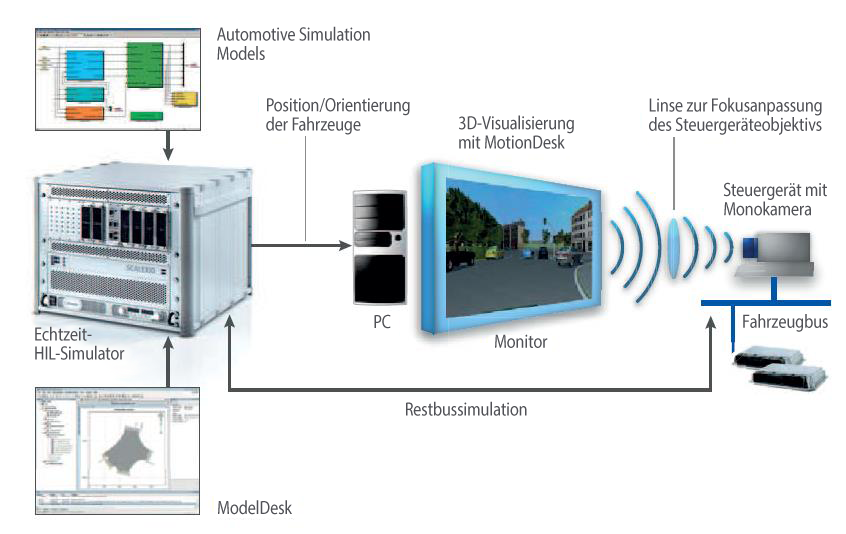
\includegraphics[width=0.8\textwidth]{images/Hil.png}
  %}
  \caption{Schematischer Aufbau eines HIL-Simulators zum Testen von kamera- und radarbasierten Fahrassistenzsystemen~\cite{dSPACEGmbH.2014}}
  \label{fig:HiL}
\end{figure}

Die 3D-Visualisierung wird auf diese Weise zu einem Teil der HIL-Simulation. Die Qualit\"at des Renderings bestimmt somit die Testaussagen \"uber die korrekte Funktionalit\"at des kamerabasierten Systems. Dies trifft insbesondere auf die Qualit\"at des verwendeten Beleuchtungsmodells zu~\cite{Nentwig.2014}.
Des Weiteren kann der Entwicklungszyklus des Fahrerassistenzsystems \"uber eine m\"oglichst realistische Darstellung verk\"urzt werden, da weniger Testfahrten mit realen Fahrzeugen unternommen werden m\"ussen~\cite{dSPACEGmbH.2013}.
